\documentclass[a4paper, 14pt]{extarticle}
\usepackage[english,russian]{babel}
\usepackage[T1]{fontenc}
\usepackage[utf8]{inputenc}
\usepackage{fontspec}
\usepackage{indentfirst}
\usepackage{enumitem}
\usepackage{graphicx}
\usepackage[
  left=20mm,
  right=10mm,
  top=20mm,
  bottom=20mm
]{geometry}
\usepackage{parskip}
\usepackage{titlesec}
\usepackage{xurl}
\usepackage{hyperref}
\usepackage{float}
\usepackage[
  figurename=Рисунок,
  labelsep=endash,
  justification=centering
]{caption}
\usepackage[outputdir=build, newfloat]{minted}
\usepackage{chngcntr}

\selectlanguage{russian}

\hypersetup{
  colorlinks=true,
  linkcolor=black,
  filecolor=blue,
  urlcolor=blue,
}

\renewcommand*{\labelitemi}{---}
\setmainfont{Times New Roman}
\setmonofont{JetBrains Mono}[
  SizeFeatures={Size=11},
]

\newenvironment{code}{\captionsetup{type=figure}}{}
\BeforeBeginEnvironment{code}{\bigskip}
\AfterEndEnvironment{code}{\bigskip}

\setminted{
  fontsize=\footnotesize,
}

\setlength{\parskip}{6pt}

\setlength{\parindent}{1.25cm}
\setlist[itemize]{itemsep=0em,topsep=0em,parsep=0em,partopsep=0em,leftmargin=2.0cm,wide}
\setlist[enumerate]{itemsep=0em,topsep=0em,parsep=0em,partopsep=0em,leftmargin=2.0cm,wide}

\renewcommand{\thesection}{\indent\arabic{section}.}
\renewcommand{\thesubsection}{\indent\thesection\arabic{subsection}.}
\renewcommand{\thesubsubsection}{\indent\thesubsection\arabic{subsubsection}.}

\titleformat{\section}{\normalfont\bfseries}{\thesection}{0.5em}{}
\titleformat{\subsection}{\normalfont\bfseries}{\thesubsection}{0.5em}{}
\titleformat{\subsubsection}{\normalfont\bfseries}{\thesubsubsection}{0.5em}{}

\titleformat*{\section}{\normalfont\bfseries}
\titleformat*{\subsection}{\normalfont\bfseries}
\titleformat*{\subsubsection}{\normalfont\bfseries}

\titlespacing{\section}{\parindent}{\parskip}{\parskip}
\titlespacing{\subsection}{\parindent}{\parskip}{\parskip}
\titlespacing{\subsubsection}{\parindent}{\parskip}{\parskip}

\linespread{1.5}
\renewcommand{\baselinestretch}{1.5}

\begin{document}

\begin{titlepage}
  \vspace{0pt plus2fill}
  \noindent

  \vspace{0pt plus6fill}
  \begin{center}
    Санкт-Петербургский национальный исследовательский университет
    информационных технологий, механики и оптики

    \vspace{0pt plus3fill}

    Факультет инфокоммуникационных технологий

    Направление подготовки 11.03.02

    \vspace{0pt plus2fill}

    Лабораторная работа №5

    <<Выражения и управление программным потоком. Построение классов>>

  \end{center}

  \vspace{0pt plus6fill}
  \begin{flushright}
    Выполнил: \\
    Швалов Даниил Андреевич

    Группа: К33211

    Проверил: \\
    Иванов Сергей Евгеньевич
  \end{flushright}

  \vspace{0pt plus5fill}
  \begin{center}
    Санкт-Петербург

    2024
  \end{center}
\end{titlepage}

\setcounter{page}{2}

\section*{Введение}

Цель работы:
\begin{itemize}
  \item создание приложений, реализующих основные управляющие конструкции;
  \item проектирование классов, взаимодействие между классами;
  \item проектирование иерархии классов для задач из различных предметных
  областей;
  \item реализация наследования и полиморфизма.
\end{itemize}

\section*{Ход работы}

\subsection*{Задание 1. Использование битовых операций}

В данном задании необходимо выполнить умножение переменной на 10, используя
операции сдвига и сложения.

Поскольку умножение с помощью битовой арифметики возможно только на степени
двойки, то необходимо разложить умножение на 10 на степени двойки. Таким
образом, умножение на 10 можно представить как сумму умножения на 8 и умножения
на 2. Для умножения на 8 необходимо сдвинуть изначальное значение на 3 бита
влево, а для умножения на 2 --- на 1 бит влево. На рисунке \ref{fig:task-1-1}
приведен исходный код получившейся программы. На рисунке \ref{fig:task-1-2}
показан пример работы программы.

\begin{figure}[H]
  \centering
  \inputminted{java}{../code/task-1/Task1.java}
  \caption{Исходный код программы}
  \label{fig:task-1-1}
\end{figure}

\begin{figure}[H]
  \centering
  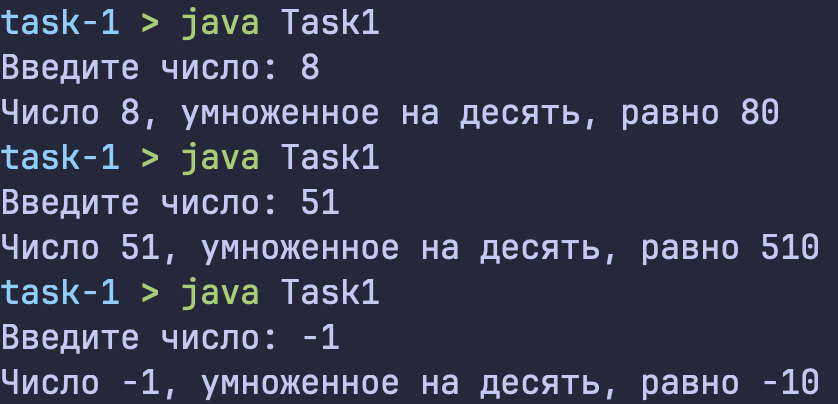
\includegraphics[width=0.7\textwidth]{images/task-1.png}
  \caption{Пример работы программы}
  \label{fig:task-1-2}
\end{figure}

\subsection*{Задание 2. Использование оператора switch}

В данном задании необходимо создать класс Date, который хранит информацию о
годе, месяце и дне. Также он должен обладать методом
\foreignlanguage{english}{displayMonth}, который возвращает наименование месяца.

В ходе выполнения задания был создан класс Date, который обладает геттерами и
сеттерами для года, месяца и дня. Каждый из них проверяет корректность
передаваемых данных. Если данные некорректны, то выбрасывается исключение. Также
был создан конструктор, принимающий год, месяц и день. Внутри он использует те
же сеттеры.

На рисунке \ref{fig:task-2-1} приведен исходный код получившейся функции
\foreignlanguage{english}{displayMonth}. В ней используется оператор
\foreignlanguage{english}{switch} для создания соответствия между числовым и
строковым представлением месяца.

\begin{figure}[H]
  \centering
  \begin{minted}{java}
public static String displayMonth(int month) {
    switch (month) {
        case 1:
            return "January";
        case 2:
            return "February";
        case 3:
            return "March";
        case 4:
            return "April";
        case 5:
            return "May";
        case 6:
            return "June";
        case 7:
            return "July";
        case 8:
            return "August";
        case 9:
            return "September";
        case 10:
            return "October";
        case 11:
            return "November";
        case 12:
            return "December";
        default:
            throw new IllegalArgumentException("Invalid month value: " + month);
    }
}
\end{minted}
  \caption{Исходный код метода displayMonth}
  \label{fig:task-2-1}
\end{figure}

На рисунке \ref{fig:task-2-2} приведен исходный код функции
\foreignlanguage{english}{main}. В ней создается дата, после чего выводится
текстовое представление месяца. На рисунке \ref{fig:task-2-3} приведен вывод
данной программы.

\begin{figure}[H]
  \centering
  \begin{minted}{java}
public static void main(String[] args) {
    Date date = new Date(2024, 7, 3);
    System.out.println("Month: " + Date.displayMonth(date.getMonth()));
}
  \end{minted}
  \caption{Исходный код функции main}
  \label{fig:task-2-2}
\end{figure}

\begin{figure}[H]
  \centering
  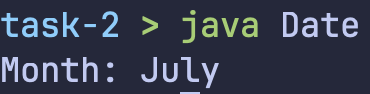
\includegraphics[width=0.3\textwidth]{images/task-2.png}
  \caption{Пример работы программы}
  \label{fig:task-2-3}
\end{figure}

\subsection*{Задание 3. Проектирование классов}

В данном задании необходимо спроектировать иерархию классов для хранения
информации о сделке между двумя участниками.

В ходе выполнения данного задания были разработаны следующие классы:
\begin{itemize}
  \item Account --- хранит информацию об участнике сделке: его фамилию, имя и
  количество денежных средств;
  \item Product --- хранит информацию о товаре: его название и стоимость;
  \item ProductItem --- хранит информацию о товаре и его количестве;
  \item Deal --- хранит информацию о сделке.
\end{itemize}

Для тестирования работы классов был написан код, представленный на рисунке
\ref{fig:task-3-1}. В ней считывается из консоли информация об участниках
сделки, а также информация о товарах. После этого сделка закрывается. Результат
работы данной программы представлен на рисунке \ref{fig:task-3-2}.

\begin{figure}[H]
  \centering
  \begin{minted}{java}
public static void main(String[] args) {
    System.out.println("Enter seller information");
    Account seller = Account.read();
    System.out.println("Enter buyer information");
    Account buyer = Account.read();

    Deal deal = new Deal(seller, buyer);

    System.out.print("Enter number of product types: ");
    Scanner scanner = new Scanner(System.in);
    int productItemsCount = scanner.nextInt();
    for (int i = 0; i < productItemsCount; ++i) {
        Product product = Product.read();
        System.out.print("Enter count: ");
        int count = scanner.nextInt();
        deal.addProduct(product, count);
    }

    deal.close();

    System.out.println("Seller money: " + seller.getMoney());
    System.out.println("Buyer money: " + buyer.getMoney());
}
  \end{minted}
  \caption{Исходный код функции main}
  \label{fig:task-3-1}
\end{figure}

\begin{figure}[H]
  \centering
  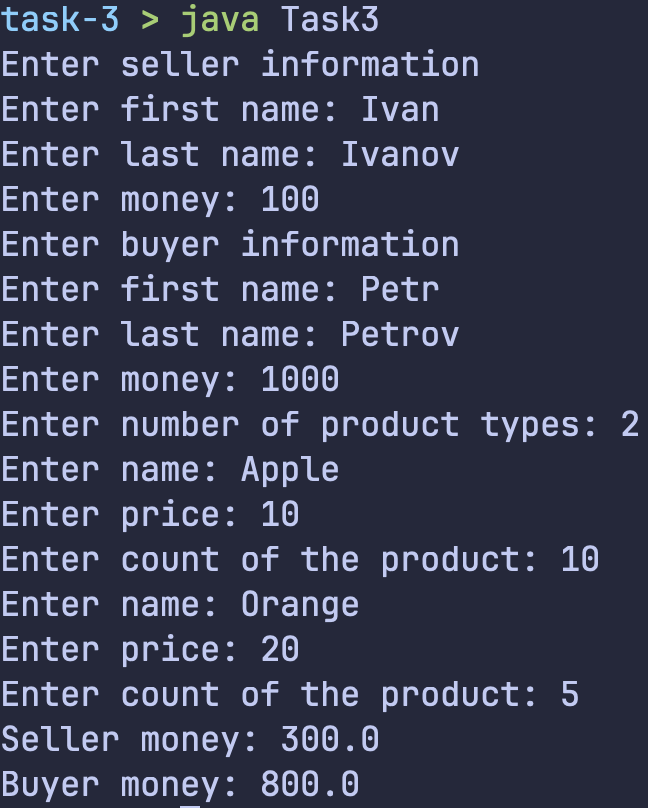
\includegraphics[width=0.5\textwidth]{images/task-3.png}
  \caption{Пример работы программы}
  \label{fig:task-3-2}
\end{figure}

\subsection*{Задание 4. Проектирование иерархии классов организации}

В данном задании необходимо спроектировать иерархию классов организации.

В ходе выполнения данного задания были спроектированы следующие классы:
\begin{itemize}
  \item Employee --- общий класс работника, содержит фамилию, имя и размер
  заработной платы;
  \item Engineer --- класс, представляющий инженера и наследуемый от класса
  Employee, также содержит квалификацию инженера;
  \item Manager --- класс, представляющий менеджера и наследуемый от класса
  Employee, также содержит список подчиненных сотрудников;
  \item Secretary --- класс, представляющий секретаря и наследуемый от класса
  Employee, также содержит информацию о начальнике;
  \item Directory --- класс, представляющий директора и наследуемый от класса
  Employee.
\end{itemize}

Все эти классы реализуют или переопределяют метод
\foreignlanguage{english}{display}, который возвращает информацию о сотруднике в
виде строки. Вызовы этого метода являются полиморфными.

На рисунке \ref{fig:task-4-1} приведен код функции
\foreignlanguage{english}{main}, с помощью которого была протестирована работа
программы. В ней создается экземпляр каждого класса, а потом вызывается функция
\foreignlanguage{english}{display}. На рисунке \ref{fig:task-4-2} приведен
пример работы программы.

\begin{figure}[H]
  \centering
  \begin{minted}{java}
public static void main(String[] args) {
    Employee employee = new Employee("Ivan", "Ivanov", 10);
    Engineer engineer = new Engineer("Petr", "Petrov", 20, 1);
    
    List<Employee> subordinates = new ArrayList<>();
    subordinates.add(employee);
    subordinates.add(engineer);

    Manager manager = new Manager("Svetlana", "Tamarova", 30, subordinates);
    Director director = new Director("Bogdan", "Ibragimov", 100);
    Secretary secretary = new Secretary("Elena", "Skorohodova", 20, director);

    System.out.println(employee.display());
    System.out.println();

    System.out.println(engineer.display());
    System.out.println();

    System.out.println(manager.display());
    System.out.println();

    System.out.println(secretary.display());
    System.out.println();

    System.out.println(director.display());
    System.out.println();
}
  \end{minted}
  \caption{Исходный код функции main}
  \label{fig:task-4-1}
\end{figure}

\begin{figure}[H]
  \centering
  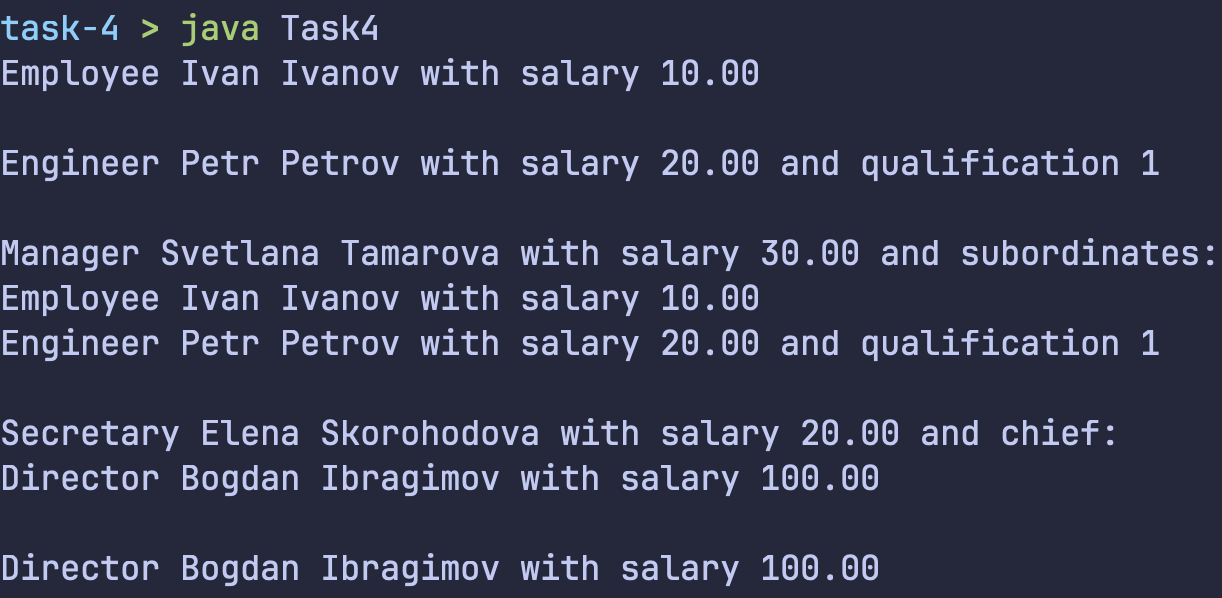
\includegraphics[width=0.6\textwidth]{images/task-4}
  \caption{Пример работы программы}
  \label{fig:task-4-2}
\end{figure}

\section*{Заключение}

В ходе выполнения лабораторной работы были созданы приложения, реализующие
основные управляющие конструкции. Также была спроектирована иерархия классов и
принципы взаимодействия между ними. В добавок ко всему, было реализовано
наследование и использован полиморфизм.

Цель, поставленная в начале работы, достигнута, задачи выполнены.

\end{document}
